\documentclass{acm_proc_article-sp}

\usepackage{graphicx}
\usepackage{lipsum}
\usepackage{listings}
\usepackage{minted}
\usepackage{amssymb}
\usepackage{setspace}
\usepackage{commath}
\usepackage{bbding}
\usepackage{hyperref}
\usepackage{graphicx}
\graphicspath{ {c:~/TwitterMining/Report/} }
\newcommand*{\field}[1]{\mathbb{#1}}%


\title{Predicting Stock Trends using Twitter Sentiment}
\author{
    Nicolas Broeking \\
    \small Department of Computer Science \\
    \small University of Colorado Boulder \\
    \small \textbf{CSCI 5502} \\
    \small nicolas.broeking@colorado.edu \\
    \and
    Anna Hoffee \\
    \small Department of Applied Math \\
    \small University of Colorado Boulder \\
    \small \textbf{CSCI 4502} \\
    \small anna.hoffee@colorado.edu \\
    \and
    Joshua Rahm \\
    \small Department of Computer Science \\
    \small University of Colorado Boulder \\
    \small \textbf{CSCI 5502} \\
    \small joshua.rahm@colorado.edu \\
}


\begin{document}

\toappear{Permission to make digital or hard copies of all or part of this work
for personal or classroom use is granted without fee provided that copies are
not made or distributed for profit or commercial advantage and that copies bear
this notice and the full citation on the first page. To copy otherwise, or
republish, to post on servers or to redistribute to lists, requires prior
specific permission..  Copyright 2015 Broeking, Rahm, Hoffee}

\maketitle

\begin{abstract} 

With social media on the rise, the amount of data available for processing is
growing at an increasing rate. It is an advanced area of research to be able to
use that data to predict or better understand the world around us. In our
project we attempted to discover a relationship between twitter sentiment and
stock values the next day. Unfortunately, we failed at determining a
relationship, but, to quote Thomas Edison, we did not fail, we found exactly how \emph{not}
to predict changes in the stock market. In addition, We were able to create a real-time
sentiment engine that allows our mobile application to get real time sentiment
analysis.

\end{abstract}

\section*{Categories and Subject\\ Descriptors}

H.3.4 [Information Systems Applications-Systems and Software]: Information
networks; J.4 [Social and Behavioral Sciences]: Economics

\section*{General Terms}
Algorithms, Measurement, Economics, Experimentation, Human Factors

\section*{Keywords}

Social Networks, Trends, Blogging, Tweets, Hashtag, Twitter, Stock

\section*{Goal}

To determine if there is a relationship between the sentiment of tweets and the
change in stock price for the next day. Then to create a user friendly mobile
application to display real time sentiment analysis.

\section{Introduction}

The recent rise in popularity of online social media has led to a huge amount
of social data available online for analysis. The popular social media site,
Twitter, gets an average of 6,000 tweets posted per second and 500 million per
day. We originally set out to determine that a relationship exists between the
sentiment of tweets and stock values for the next day. For the purposes of
this project we looked at four companies, Amazon, Apple, Google, and Samsung. 

The first step in determining a relationship was to collect data. To do this we had to gather information
from two sources, Twitter, and Yahoo. Twitter allowed us to open a connection
to the streaming API. Using this API we receive anywhere between 1\% and 40\%
of all the tweets being tweeted at any given time of the day. This percentage depends on the current Twitter
load and how many things we are filtering on. Once we received a tweet we would
store it in a database for latter processing.  In addition to collecting
twitter data we also collected historical stock data. Yahoo provides historical
stock data for companies going back many years. Once we collected all our
tweets we gathered the stock data for the same intervals of time.

Once we had all the data, we had to pre-process it before we could do any
analysis. Each dataset needed to be pre-processed in order to perform
efficient analysis. For Twitter we had to filter each tweet and
remove all unnecessary words. We needed to try to strip down the information
as much as possible or else the classifier would become unreasonable slow. The
stock data was another challenge all together. Since the tweets were not
received on a constant time bases, we had to filter all the stock data to match
up correctly with tweets. Once we preprocessed, we were then able to pass them to
the sentiment analysis step.

Before we could actually determine the correlation between the data sets, we had
to classify all the tweets.  To do this we used a Naive Bayes Classifier. Our
classifier was built to extract each word from the preprocessed text. Each word
was then added to a dictionary to describe the sentiment of each tweet.
This phase our project easily took the most time and effort. We attempted to
build the most accurate classifier and experimented with different types of
feature vectors. We discovered classifying on words yielded the best results.

Once we had the sentiment for each tweet we ran multiple tests to determine the
correlation.  The tests were mostly based off a linear regression model fitted
to the data with Ordinary Least Squares estimators. The model was not at all
adequate, but allowed us to perform many conclusive statistical tests for
correlation including a t-test and $R^2$ value examination. 

Once we determined there was no correlation, we had to decided what our
next step was. Originally, We were hoping to find a correlation but because we determined
that there wasn't one we were no longer able to create a mobile app
that predicted stock trends. However, it is still very useful to have a
sentiment analyzer so we decided that it would be best to create an mobile application to
shows sentiment analysis instead. To do this we had two parts: The REST API
and the mobile application. The REST API was written in Haskell and performed the real
time sentiment analysis.  The mobile app was written for android and reaches out
to the REST API in order to get the sentiment. The two work together to create a user
friendly, easy to use application.


\section{Authors}

The authors of this project are Nicolas Broeking, Anna
Hoffee, and Joshua Rahm. Broeking and Rahm are graduate students at the
University of Colorado at Boulder. Hoffee is an undergraduate student at the
University of Colorado.

Nicolas Broeking has worked on embedded systems and mobile applications for
the past four years. Broeking's contributions were in the data collection,
preprocessing, sentiment analysis, optimizations, and creation of the mobile
application. 

Josh Rahm has spent his career working with embedded devices, cellular
technologies and billing platforms. Rahm contributions were with sentiment
analysis, optimizations, and converting the tools to be used in a real time
system on the server. He also created  the Rest Api that allows the mobile app to get
the real time sentiment analysis.

Anna Hoffee is a student in the mathematics department. She has spent her
career working on similar projects attempting to find patterns in other live
data sets. Hoffee contributed by taking the sentiment data and determining that
there was no correlation.

\section{Motivation}

The Stock Market is one of the largest entities in Western and World economies.
In a world where a 15\% increase is assets per year is massive,  even the
ability to increase certainty in the market by a few percentage points is appreciable.
Companies and individuals can harness this technology make billions and secure
investments, producing and saving billions for the economy. While making
billions is outside the scope of this project, we thought it was possible to
significantly increase the accuracy of stock predictions. We know that public
image is critical to stock value; therefore, we predicted that if a company's
public sentiment, displayed on Twitter, were to decrease, then it would stand to reason
that there would be a drop in the stock value of said company. This ended up to be an
incorrect prediction and we were able to show that there exists no correlation
between twitter sentiment and changes in stock value.

Even with this failure, we still have motivation for sentiment analysis.
Companies still have an interest in a positive public image. There are many
ways for companies to get this information but none are as convenient as having
a phone in your pocket that easily shows you this information. The need for an
app like this was the motivation for us to take our original tools and
customize them to do real time analysis. 

\section{Literature Survey}

Many similar experiments have been done in the field of data mining. The first
and probably the closest to our project is Correlating Financial Time Series
with Micro-Blogging. This project looks at 150 random companies stock prices
over a six month time period. Then they take all the tweets with specific
hashtags related to the company and construct a context graph. In this graph
the tweets themselves were nodes and any actions on the tweets were edges. They
then use this graph to find relationships with the stock price. This project
looked for other things than just stock trends though. They wanted to find
relationships between the data and how much a stock will change, and what the
values of the stock will be. They determined that the most reliable way to
determine the information is by looking at the number of edges in the graph.
However, even in this case however they were not able to find a reliable
correlation but they did give us a start with where to begin our search[1] 

Another team, Twitter Mood Predicts the Stock Market, attempted to determine
how twitter mood affects the stock price. They grouped tweets into 6
dimensions Calm, Alert, Sure, Vital, Kind, and Happy. Then they took these
categories and created a relationship between to the closing value of the Dow
Jones. They only wanted to determine though if there was a relationship at all. 
On a very specific data set they were able to find a correlation between the values
however on a large scale their data did not work out. They showed very similar
results to what we showed. d[2] 

Many other studies have been done similar to the first two on how to use
twitter to predict stock prices. The one thing that has been determined for
sure is that there is a high correlation between peoples' attitudes and stock
value. However, it hasn't been determined if twitter accurately reflects market
sentiment and therefore is the basis of our project. In one situation Twitter
was used in 2013, to predict a drop in Royal Caribbean's stock value when
people started tweeting about the flu spreading on one of its cruises.
Researchers were able to predict the drop in price 48 minutes before the stock
plunged about 3\%. This was only a rare case however and worked under a very
specific set of circumstances.[3]

Once we found information regarding other studies that have been done in
sentiment analysis and stock price correlation we started looking into the best
ways to actually do sentiment analysis. After the midway presentation, we were not happy
with our accuracies. We talked with Jamie Wood from Waylin. Waylin specializes
in performing sentiment analysis at an industrial scale. Sentiment analysis on
twitter data is a very challenging task because tweets are a form of natural
language. Mr. Wood advised us that a 65\% accuracy is something that is
considered to be a good analyzer and any point upwards of that is a great
classification. Using this information we set a goal to achieve an accuracy
upwards of 65% [4].

We also used several blogs online from software engineers who have performed
Twitter sentiment. [5][6] They provided a good starting place for us to easily learn
the language and the toolkit before creating our own custom sentiment analyzer. 

\section{Tasks}

In order to successfully prove or in our case, disprove, a correlation and then
to create an application we split our project into ten different sub tasks.
These tasks, explained below, allowed us to split the workload among the group
and to ensure that we stayed on a schedule for a successful project.

\subsection{Data Collection} 

To collect all the data that we needed to get it from two sources.
First we had to get a decent volume of tweets to perform the sentiment
analysis. Then we had to gather data from Yahoo that matched the same time
period os the twitter data.

\subsubsection{Twitter Collection} 

In order to collect the tweets from Twitter we needed to set up a channel to
the Twitter Streaming API. The API allows us to request all tweets related to
Amazon, Apple, Google, or Samsung. Depending on the current load to the twitter
servers this provided anywhere from 4\% to 40\% of all tweets being posted at
any given time. In order to create the streaming tool we used python and a library
called Tweepy. Tweepy allows a call back event system that will notify everytime
Twitter has more tweets for us. 

Once we had the tweets we immediately stored them in a SQLite database.  We had
a lot of discussion about what would be the best way to store the tweets. We
had to make sure that we kept up with the streaming API or else twitter would
block our connection. SQlite is a lightweight fast database that is reliable
and easy to use. We also didn't have to worry about other processes attempting
to access the same service so SQLite seemed like a great choice. For each tweet
we stored the text, its retweeted count, time of the tweet, userid and the
tweet id. For each user we also stored the userid, the followers count, friend
count, and their name. We ended up not using all this information but we wanted
to store all relevant information during the data collection phase so we would
have it just in case it became relevant later. 

Every time we received a tweet from twitter a callback was called that allowed
us to put it in the database. This function is shown below.

\inputminted{python}{examples/streaming.py}

\subsubsection{Stock Collection} 

To get the stock data we needed to collect historical data fore each of our
four companies. Yahoo Finances has a great API that allowed us to download the
data at the day granularity going back a couple years. We only took the data
for the same time period as our tweets and then stored them in a comma
separated text format.  This data source provides us with the Open, Close,
High, Low, and Data attributes. Similarly, to the tweets, we stored more
information than we needed to make sure that we had extra information in case
we needed it. 

\subsection{Data Preprocessing}

The preprocessing step, like the data collection step, was done in two parts.
First we did the preprocessing of the tweets to prepare for the sentiment analysis.
Then we preprocessed the stock data to fit with the twitter data to allow us to 
compare between the two data sets.

\subsubsection{Tweet Preprocessing}

Our twitter preprocessing step went through many versions of development before
it arrived in its current state. In the first version we removed all words
under three letters and then passed on the full tweet to the classifier.
Unfortunately, this did not give us any good results. There were too many words
to add to our feature vector and so we ended up with a lot of irrelevant
features. The next iteration of the project used a different feature extractor.
In this step we refactored our pre processor to strip away all non alpha
characters. 

Finally, before the midway presentation we refactored again to a
more complex pre processor. In this version we removed all urls and replaced it
with the string URL. Then we tool all hashtags and replaced it with the string
TAG. After the feedback from the midway presentation we decided that we weren't
satisfied with our pre processor and so we did research. We added other
functions that allowed our preprocessor to become the most effective. The first
major thing we did was to replace all repeating characters with two of the same.
In the tweet "I loooooooooooooove hamburgers" compared against "I looooove
pickles" we would get two different words for love. We really only want one
though because they represent the same word. 

Our first pre processor step would
change this to "I loove hamburgers" The first logical question is then why do
we leave two o in the word. This is because people use repeating characters to
stress emotion so we want to treat loove and love differently. In addition to
this we also changed all the characters to lowercase, changed any username to
AT\_USER, removed additional white space, and stripped any punctuation. The
code for these two steps is shown below.

\break
\inputminted{python}{examples/preTweet.py}

After these two steps, we also filtered out any stop words. Stop words are a
list of words that are proven to have no sentiment value but will sway the
classifier. The combination of all these steps brought us to our final pre
processor.

\subsubsection{Stock Preprocessing}
 
The last step in pre-processing, after sentiment analysis was performed on the
tweets, was to combine the twitter data with the stock data. Since the two came
from very different sources and in different formats work had to be done before
they could be combined for correlation analysis. The goal was to calculate the
change in stock value from day $n$ to day $n+1$ and pair it with the percent of
positive tweets on day $n$, This proved to be not straightforward due to the
fact that there were arbitrary sized missing blocks of days in the twitter
data, as well as no stock data on weekends. A day of twitter data had to be
thrown out if there wasn't stock values available for that day and the
preceding, and stock values had to be thrown out if their wasn't the
appropriate twitter and additional stock data to go along with it. A function
to determine weather or not two days are one day apart aided a lot in the
pre-processing:

\break 
\begin{minted}{R}
one.day <- function(date1,date2) {

  daysPerMonth <- c(0, 31, 28, 31, 30, 31, 
                    30, 31, 31, 30, 31, 30, 
                    31)
       
      month1 <- as.numeric(date1[2])
      day1<- as.numeric(date1[3])

      month2 <- as.numeric(date2[2])
    day2 <- as.numeric(date2[3])

    if (abs(month2 - month1) > 1){
        return (0)
        }

    if(month1 == month2){
        if(abs(day2-day1) > 1){
            return (0)
              }
        else{
            return (1)
             }
       }
    lastDayMonth1 = daysPerMonth[month1]
    lastDayMonth2 = daysPerMonth[month2]

    if(day1 == lastDayMonth1 && day2 == 1){
        return (1)
         }
    if(day2 == lastDayMonth2 && day1 == 1){
        return (1)
        }

    return (0)

}

\end{minted}

After the stock and twitter data was converted to the same format and
reorganized into consecutive days the correlation analysis could begin. 

\subsection{Sentiment Analysis}

After creating the Preprocessing tools, we created the sentiment analyzer.  We
wrote the sentiment analyzer in python using the natural language tool kit
library. In the final version we trained the classifier on 15000 tweets and
then test its accuracy with 10000 tweets. Like the preprocessing step this
phase went through a few iterations as well. We started with basic classifier
and ended up with a high performing Naive Bayes Classifier that performed in
real time.

The major part of the sentiment analysis was choosing features to use for our
classifier. At first we just looked at raw words. However, with our less than
good pre processor we weren't able to get reasonable results. In this first
version we were only able to train on 2000 tweets because our memory got so
bloated that training on anymore would cause the process to get killed. The
accuracy in this step lied somewhere between the 50\% and 55\% mark. In order
to try to create a better classifier we attempted to try other features. We
found examples of people using letters to classify gender of a name and thought
we could apply this to our classifier. We turned out to be very wrong. Our
letter classifier showed about a 50\% accuracy. This is about the accuracy we
would expect to see if we were to randomly guess. After this slight set back, we
went back to the drawing board.  We talked with a Jamie Wood from Waylin.
Waylin specializes in twitter sentiment and provides similar services to their
customers. Mr. Wood told us that a 65\% accuracy would be considered a very good
accuracy and anything above that would require a much larger training set.
After talking to Mr. Wood we refactored again to use words as features but
created a smarter feature extractor, shown below, that utilized the new
preprocessing steps.

\inputminted{python}{examples/featureExtractor.py},:

As a Part of the new steps we also improved the training data that we fed to the
classifier.  We made sure to have the same amount of positive tweets as
negative tweets and we applied the new pre processing steps. In our final
version our training looked like below.

\break
\inputminted{python}{examples/train.py}

The new feature extractor worked really well with an accuracy at about 64\% but
still wasn't as good as we wanted. We realized the problem was most likely with
the slowness of our code. We then spend the next week attempting to optimize it
even further. We started by using sets instead of lists and then using these
sets to reverse how we were determining the feature vector. By iterating on the
tweets instead of the feature vector and by using a dictionary with default
values we were able to speed up the performance of our code by about 1000
times. At the midway demo we were processing about 5 to 10 tweets a second.
After our optimizations we started classifying over 4000 tweets per second.
This brought our runtime from about $O((nm)^2)$ where n is the number of tweets
and m is the words in each tweet, to $O(nm)$ These optimizations then allowed
us to train on 15000 tweets instead of just 5000. The extra volume of training
jumped our accuracy up to about 90\%. This was a huge success in the project
because the jump in accuracy allows for us to find the correlation with a much
higher accuracy. 

When we brought our classifier to the full dataset, we ran into one more
problem.  Previously when we were running our classifier we did it on such a
small database that we could fit it all into memory. However, when we stepped
up the full dataset the operating system would start killing our process
for using so much memory. This led to the last optimization we had to do on our
classifier. We used a generator on the SQLite database to only return 1000
stored tweets at a time, shown below. These optimizations dramatically
increased the effectiveness of our classification step.

\inputminted{python}{examples/generator.py}

The final piece of our classifier was putting it all together. After training
our classifier we needed to read all the stored tweets from the database and
export them to a comma separated list for the Correlation analysis. To do this
step we had a function that read from the database and echoed the tweet into
the correct company bin.

\inputminted{python}{examples/converter.py}

This classifier was able to sort all of our 10 gb of tweet data into the
separate company bins in about 10 hours using 3 different processes. 

\subsection{Correlation Analysis}

After the sentiment analysis is completed and we had all the tweets
classified as positive or negative we could begin the correlation analysis.

We were then able to graphically examine the relationship between
the percent of positive tweets and the change in stock price. As well, we well
perform a few different statistical tests to determine if there is any use full
correlation. \newline\textbf{  Test One: Linear Regression} \newline\indent
Assume $ y = \beta_0  + \beta_1x\ \ \  $ where y = change in stock value, x =
percent of positive tweets. I'll use the Ordinary Least Squares estimators to
derive the regression parameters. To use OLS estimators we assumed that
there was a linear relationship between response variable and the regressor. We
also assumed that the residuals of this model will be uncorrelated and
have constant variance. The $lm()$ function in R will perform the regression.


Regression models for open and close values for each company were created and
all came out with very similar results.  One example, change in
Google Open values regressed on percent of positive tweets: \newline\indent
$\hat{Y} = -2.48 + 6.794 x$the \newline\indent and the model summary is:

\begin{minted}{R} 

lm(formula = open.vec ~ percent.pos)

Residuals:
     Min       1Q   Median       3Q      Max 
-12.4474  -2.1983  -0.3133   3.1269  13.2047 

Coefficients:
            Estimate Std. Error t value Pr(>|t|)
(Intercept)   -2.480      8.597  -0.289    0.776
percent.pos    6.794     18.524   0.367    0.717

Residual standard error: 5.392 on 22 degrees of freedom
Multiple R-squared:  0.006077,  Adjusted R-squared:  -0.0391 
F-statistic: 0.1345 on 1 and 22 DF,  p-value: 0.7173

\end{minted}

\indent Then we did a hypothesis test, specifically a T-test, to see if
$\beta_1$ should equal 0, this would indicate that there is no relationship
between $x$ - percent of positive tweets, and $y$ - change in stock price. We
set $\alpha = .05$ meaning that theoretically $5 \%$ of the time we
would reject the null hypothesis $ (H_0)$ in favor of the alternate hypothesis
$(H_1)$ when $ _0$ is actually true.  

\indent $ H_0: \beta_1 = 0 \ \ \
H_1: \beta_1 \neq 0$ \newline\indent\large $T_{calc} = \frac{ \hat{\beta_1} - 0
}{s.e.(\hat{\beta_1})} = \frac{6.794}{18.524} = 0.367 $ \newline\indent $ t_{
(n-2,\alpha/2)} = 2.07$ \newline\indent $ \abs{T_{calc}} < t_{ (n-2,\alpha/2)}
\ \ $ \normalsize so we fail to reject the null hypothesis that there is no
relationship between positive tweets and changes in stock price.

\indent In the model summary given above the p-value for $\beta_1$ is
.717. This means that for us to reject the null hypothesis that $H_0 =0$ we
would have to set $\alpha = .717$ meaning would have had to allow the test to
reject the null hypothesis when it's true $71 \%$ of the time. This is unheard
of.

\indent As well, given in the model summary is the $R^2$ value.
This measures the percent of variance in $y$ that is explained by $x$. In a
perfect linear model it would be 1. In our mode it is $.006$, indicating that
$.6\%$ of the variance in the stock price can be explained by twitter data.
This is an extremely low $R^2$ value. As well as quantitive evidence there is
qualitative evidence of an absence of linear relationship between $x$ and $y$.

See the graphs below. Note that the blue data points/regression lines
correspond to the change in close values, and the red data points/lines
correspond to the change in stock open values.

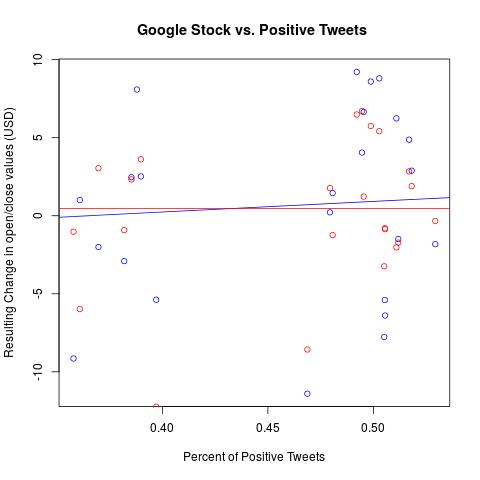
\includegraphics[scale=.5]{google_positive.jpeg}

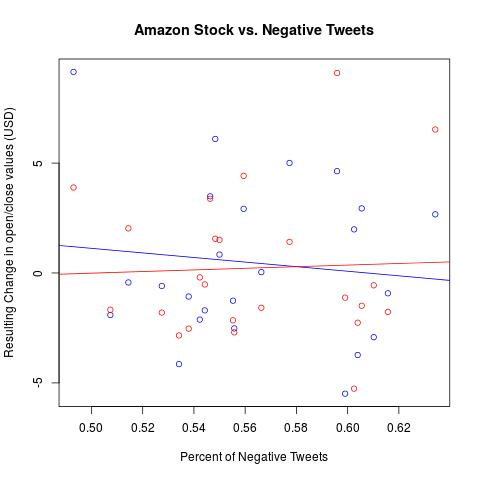
\includegraphics[scale=.5]{amazon_negative.jpeg}

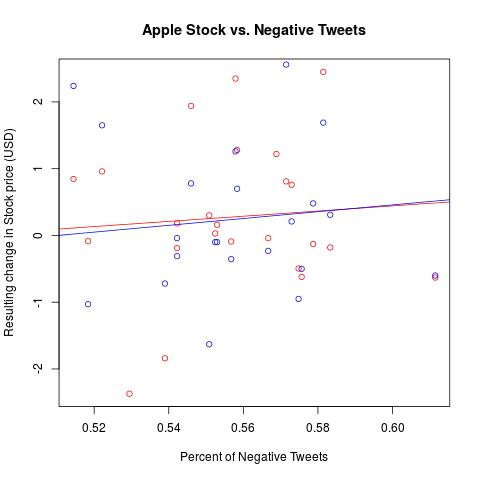
\includegraphics[scale=.5]{apple_negative.jpeg} 

\indent from these graphs it's very clear that there is no relationship between x and y.


\textbf{Test Two: Correlation Coefficient}
Cor$(X,Y) = \frac{E ( X - \mu_x)(Y - \mu_y)}{\sigma_x\sigma_y}$


This tests for linear correlation between x and y. If the correlation
coefficient is $-1$, the variables are perfectly negatively correlated. If
it is 1 then they are perfectly positively correlated.  

For Apple stock the correlation between the open values and the percent of positive
tweets is $0.079 $. This indicates that there is little to no relationship
between the two. 

\subsection{Accuracy and Error Analysis}
To evaluate the accuracy of the model we looked at the $R^2$ value, which shows
the percent change in $Y$ that is explained by $X$. We can also look at the
standard errors the of regression coefficients and the residuals of the models.
If there is much correlation in the errors we can try using the generalized
least squares estimators instead. 

It's clear that our original goal of predicting the stock market with twitter sentiment 
was not achieved. We may have gotten these results because we did not split up the data 
enough into sub-categories. We might have found more interesting patterns if we had split tweets
up into categories based off what else was in the tweet about the company, i.e. look at all the
tweets about a new product that Google/Amazon/Samsung/Apple came out with. We could have performed data mining
on the positive and negative tweets to see if there were any similarities between them (other 
than positive/negative words). Sometimes when too much data is meshed together patterns are masked;
we don't know if this did or didn't happen. This is clearly a place that our project could be extend for future work.
It is hard to be able to detect every pattern out there. We only looked at one specific pattern and just because
the one we were looking for didn't exist it doesn't mean there are not others out there that would prove to have a correlation.  

\subsection{Application}

Even though we were not able to determine a correlation between the data sets, it
didn't mean that we didn't have useful tools. Companies are still very
interested in what their company looks like in the public eye even if it
doesn't have a direct relation to their stock price. There are a lot of complex
tools out there that can help a CEO but nothing that is quick and easy and fits
in his pocket. To do this we created an application that does just this. We can
analyze the sentiment of these companies in real time and then display that
information to the user. In order to do this we have two parts. The server side
that does real time sentiment analysis and hosts a rest API for devices to use.
The mobile side is the client side that allows users to see the sentiment in
real time.

\subsubsection{Rest API}

The REST API is an application written in Haskell and Python in two distinct parts. The
Python section is responsible for collecting and analyzing incoming tweets. It then broadcasts
that information on a UDP socket. The Haskell side collects the data from the UDP socket and
is responsible for aggregating and storing the data as well as maintaining a HTTP service that
responds to a GET request and regurgitates the necessary information in JSON form.

\subsubsection{Mobile Application}

We built the mobile application for the android system. We can run it on any
android device that runs Android Lollipop or greater. This gives the user a lot
of flexibility. It is really easy for anyone to install the application to their phone
and instantly get real time sentiment analysis. When the phone starts up, it
reaches out via a web request the Rest API that is doing the sentiment
analysis. It gets the JSON back and parses it for the values. It then
calculates the percent positive and uses that to update its GUI. For the GUI we
chose to display a smiley face for a positive sentiment and a frowny face for a
negative sentiment. A screen shot of the application running in the android simulator
can be seen below.  

\break

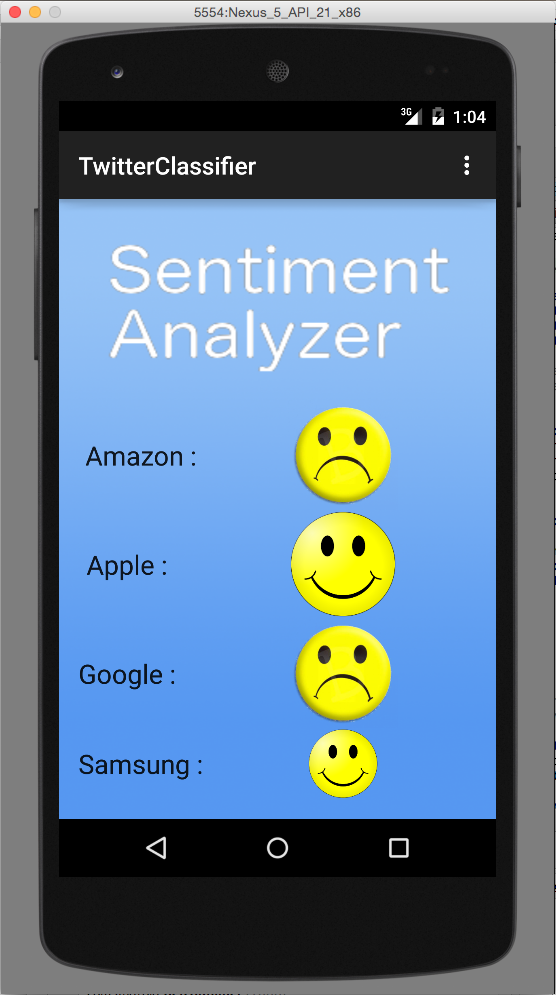
\includegraphics[width=\linewidth]{android.png}

\section{conclusion}

In conclusion we were able to determine that there is no relationship between
twitter sentiment and the change in stock price the next day. The stock market
is a complex system that is clearly not influenced by just one thing. Our calculations
showed that less than 1\% of the change is stock value could be predicted using our
methods. 

Even though we weren't able to find a relationship our project was still a success.
We were able to turn our sentiment analysis into a real-time tool that allows anyone
to open up their phone and get real-time sentiment analysis. 

Through this data mining process we learned many things about mining for sentiment.

1) Your preprocessing step must be tailored to your data. At first we were just doing
minimal work with our preprocessing and letting the classifier do most of the work. 
This however proved to be very inefficient in both time and accuracy. Getting to know
the data and then removing the stuff that you don't need proved to not only speed 
up the classifier but also to provide more accurate results.

2.) Feature extraction is the key to a good Naive Bayes Classifier. If you choose
the wrong features you just wont get accurate results. In addition to the accuracy
if you are inefficient in your feature extraction it will bog down the whole system. 

3.) Just because you don't find a correlation doesn't mean that the project is a failure.
We were able to prove that there is no correlation which helps further research in 
the area. This also led us to be able to create a useful app that shows real time 
sentiment analysis

\section{Future Work}

In our project we determined that there is no correlation between stock and
twitter sentiment on a day by day basis. This does not rule out many other
granularities though.  One could potentially find a relationship hour to hour,
minute to minute, week to week, or even year to year. There are so many
timeframes that could be researched that we were not even able to scratch the
surface on what is possible. In future work more research should be done to see
if one could predict stocks on another level. 

Even though we found no correlation to be able to predict stock prices that
doesn't necessarily mean there is no value in knowing the sentiment of a
company. One might be able to discovery that only very large changes in
sentiment can detect a change in stock prices.  It was already shown from other
studies that researches were able to see a dip in the stock price by watching
what was being posted on twitter. It would be interesting to investigate
phenomenon such as this more in depth.  

\section{Sources}

1.) Eduardo J. Ruiz, Vagelis Hristidis, Carlos Catillo, Aristides Gionis, and
Alejanro Jaimes,  2012, Correlating Financial Time Series with Micro-Blogging
Activity DOI=http://www.cs.ucr.edu/~vagelis/publications/wsdm2012-microblog-financial.pdf 

2.) Johan Bollen, Huina Mao, Xiao-Jun Zeng, 2010, Twitter mood predicts the stock
market, arXiv:1010.3003 [cs.CE], DOI=http://www.sciencedirect.com/science/article/pii/S187775031100007X


3.) Stan Alcorn, Twitter Can Predict The Stock Market, If You're Reading The Right
Tweets, 2013

4.) http://ravikiranj.net/posts/2012/code/how-build-twitter-sentiment-analyzer/

5.) http://www.labic.icmc.usp.br/wti2010/IIIWTI\_camera\_ready/74769.pdf

6.) http://thinknook.com/twitter-sentiment-analysis-training-corpus-dataset-2012-09-22/

7.) https://snippetsofcode.wordpress.com/2014/04/28/fast-tutorial-to-nltk-using-python/

 \end{document}
